% %%%%%%%%%%%%%%%%%%%%%%%%%%%%%%%%%%%%%%%%%%%%%%%%%%%%%%%%%%%%%%%%%%%%%
% %% SpDCache %%
% Reduction Cache
% %%%%%%%%%%%%%%%%%%%%%%%%%%%%%%%%%%%%%%%%%%%%%%%%%%%%%%%%%%%%%%%%%%%%%

\section{Reduction Cache}
\label{sec:spdc:redc}

\lettrine{P}{erforming} a \gls{reduction} in hardware requires a read from memory, followed by an accumulation and a write back.
This operation is denoted $\mathit{RED}(key, value)$~\cite{Srikanth2021_SortCache} with the \emph{key} being the position in the output vector $c$.
In Figure~\ref{fig:spdc:GC_cache_WB}, we show three cases that occur in a generic data-cache when a \gls{reduction} is performed.
If the vector entry ($c_{key}$) \glspl{hit} in the cache, the \emph{update} is performed by the processor (in \textit{red}) with no external memory access (on the left in the figure).
When there is a \gls{miss}, the operation is blocked until the read from main memory completes (in the middle of the figure).
Potentially, the \gls{miss} will also trigger an \gls{eviction}, which exacerbates the blocking condition, because a cache-line must first be written back, before the read from main memory can be performed (on the right in the figure).
In scientific applications, the matrices are extremely large and only a small portion of the vector $c$ can reside in the cache, thus the \emph{miss+evict} case arises frequently.

A \gls{redC}, such as~\cite{Srikanth2021_SortCache} or~\cite{Mukkara2019_PHI}, is a data-cache which accepts \gls{reduction} instructions (\emph{RED}) from the processor and performs accumulations locally (near-memory).
In the case of a \gls{hit}, see Figure~\ref{fig:spdc:red_based_cache}, the \gls{reduction} takes place in the cache (in \textit{blue}, on the left in the figure).
For a \gls{miss}, the cache allocates a new line with zeros, and simply inserts the value (in the middle of the figure).
In this case, the cache-line is inconsistent with main memory.
Only when the line needs to be evicted, is a read performed (on the right in the figure).
In the cache, the values in the line are accumulated with the main memory data, and the result is written back.

As seen in the figure, a \gls{redC} reduces the number of main memory accesses in the case of a \gls{miss}.
Instead of having the classic ascendant policy where data is stored in the cache to be pulled-up again by the processor latter-on, the \gls{redC} has a descendant policy: data is written/updated in the cache to be pushed-down to memory latter-on.
Instead of two memory transactions that can stall the processor, the \gls{redC} only needs a single ``fire-and-forget'' instruction, meaning it can be issued without waiting for an answer, thus avoiding stall issues.
At the end of the algorithm, the \gls{redC} must be flushed.

\begin{figure}[htbp]
    \centering
    \begin{subfigure}[t]{0.55555556\linewidth} %55/99
        \centering
        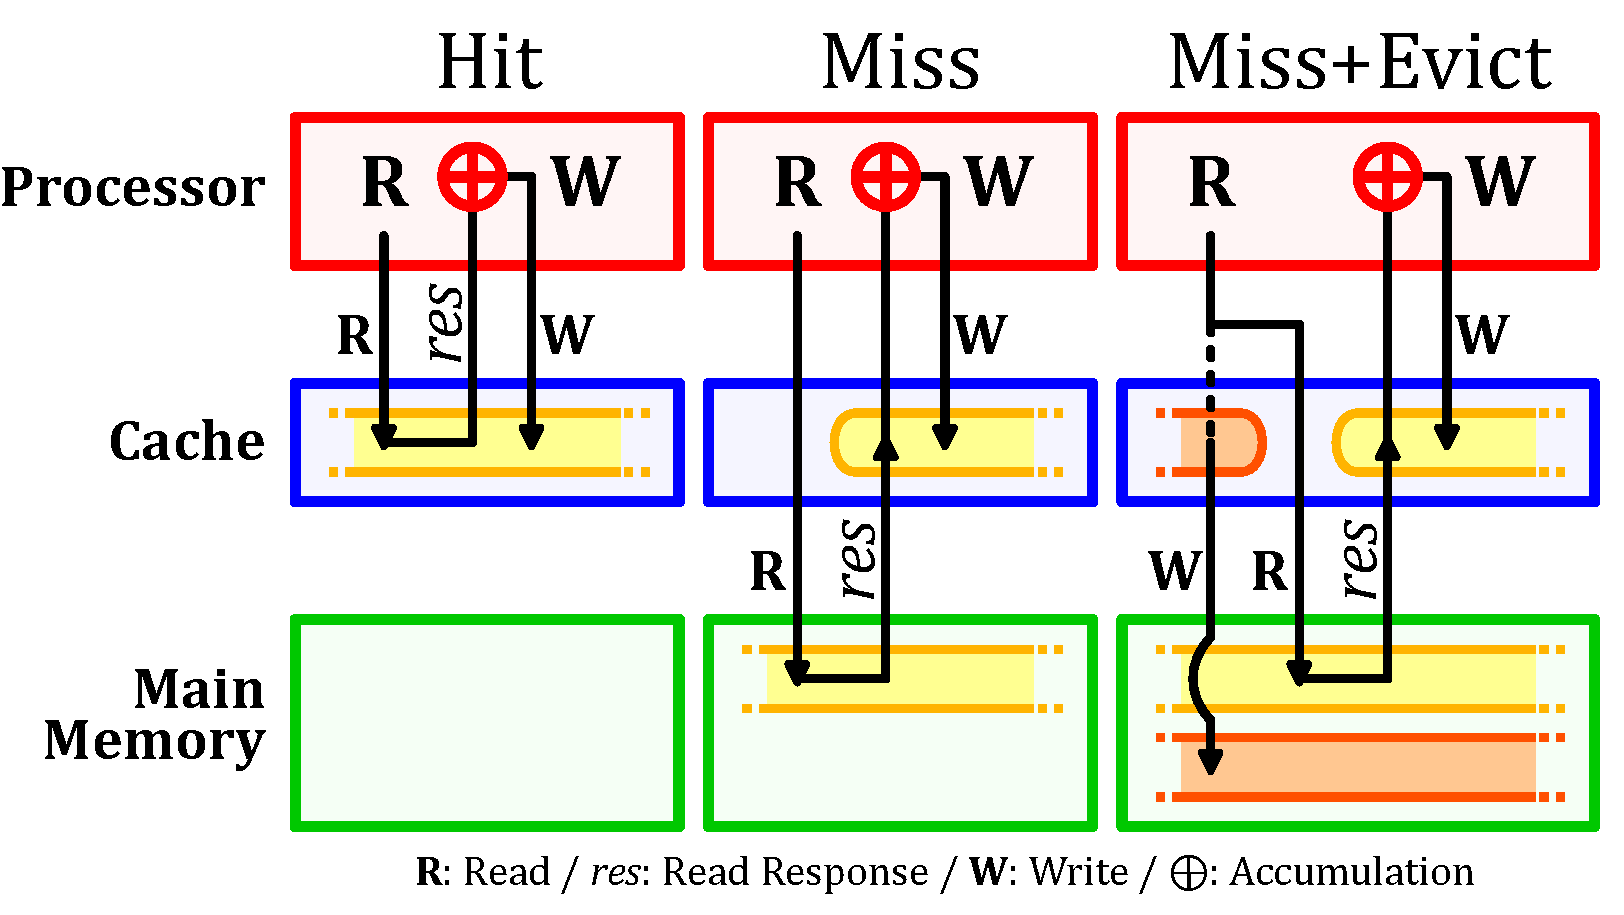
\includegraphics[width=\linewidth]{Chapter_SpDC/Figures/PDF/GCvsRedC_00.pdf}
        \caption{Generic Cache (Write-Back)}
        \label{fig:spdc:GC_cache_WB}
    \end{subfigure}
    \hfill
    \begin{subfigure}[t]{0.41414141\linewidth} %41/99
        \centering
        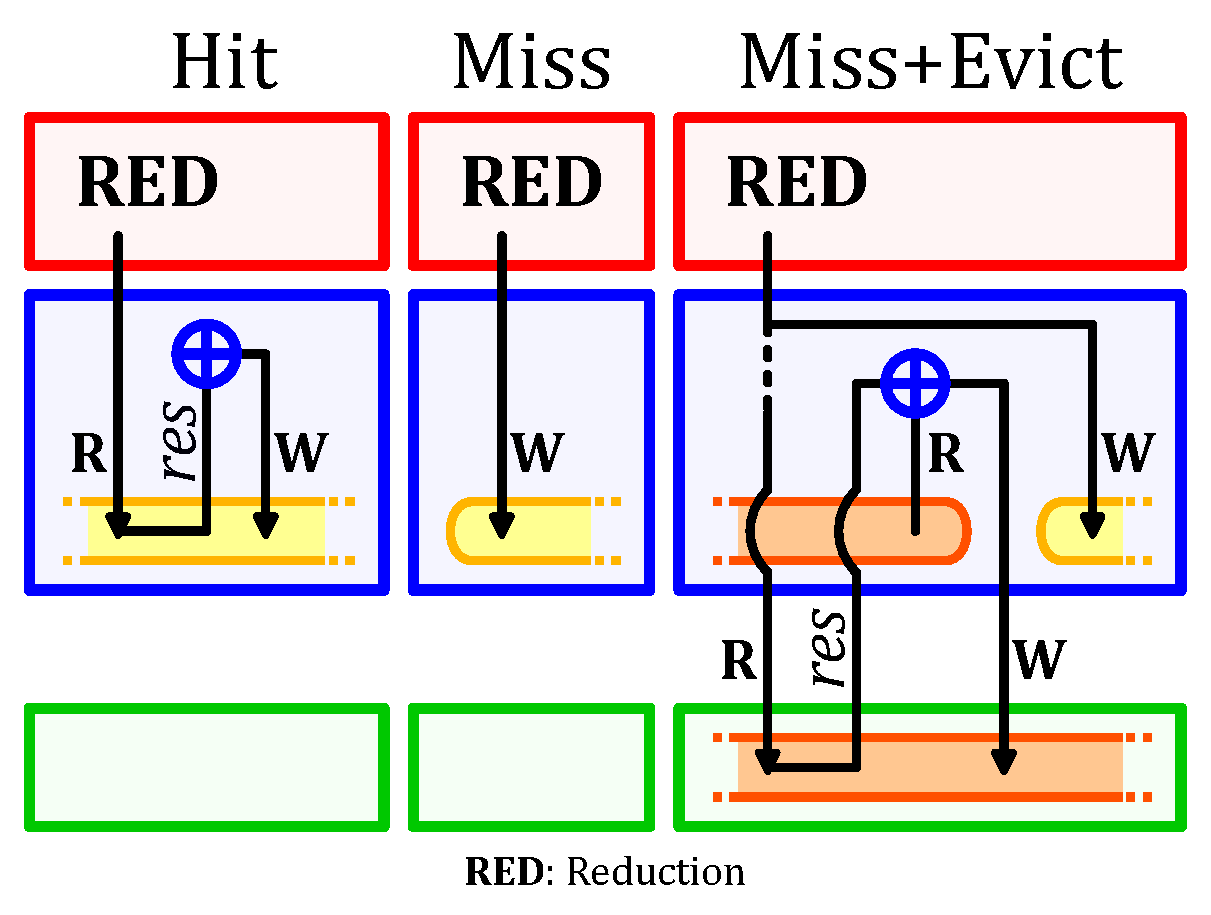
\includegraphics[width=\linewidth]{Chapter_SpDC/Figures/PDF/GCvsRedC_01.pdf}
        \caption{Reduction Cache}
        \label{fig:spdc:red_based_cache}
    \end{subfigure}
    \caption{Read (R) and Write (W) Transactions of a \Gls{reduction} Operation in Generic and \Gls{reduction} Caches}
    \label{fig:spdc:RWtransactions}
\end{figure}

\begin{highlight}{Definition}{LimeGreen}
    A \textbf{\gls{redC}} is a data-cache containing an arithmetic unit and a dedicated support for \gls{reduction} operations, via single ``fire-and-forget'' \emph{RED} instructions.
\end{highlight}

\begin{highlight}{Conclusion}{Red}
    In order to process efficient \gls{reduction} operations, a \textbf{\gls{redC}} can be used to \textbf{avoid unnecessary memory transactions and stalls}, by offloading the accumulation near-memory, and updating the main memory only at \gls{eviction}.
\end{highlight}